\documentclass{standalone}
\usepackage{pgfplots}
\pgfplotsset{compat=1.18}
\usepackage{amsmath}
\usepackage{xcolor}

\definecolor{toneBlue}{HTML}{1565c0}
\definecolor{selfOrange}{HTML}{e65100}

\begin{document}
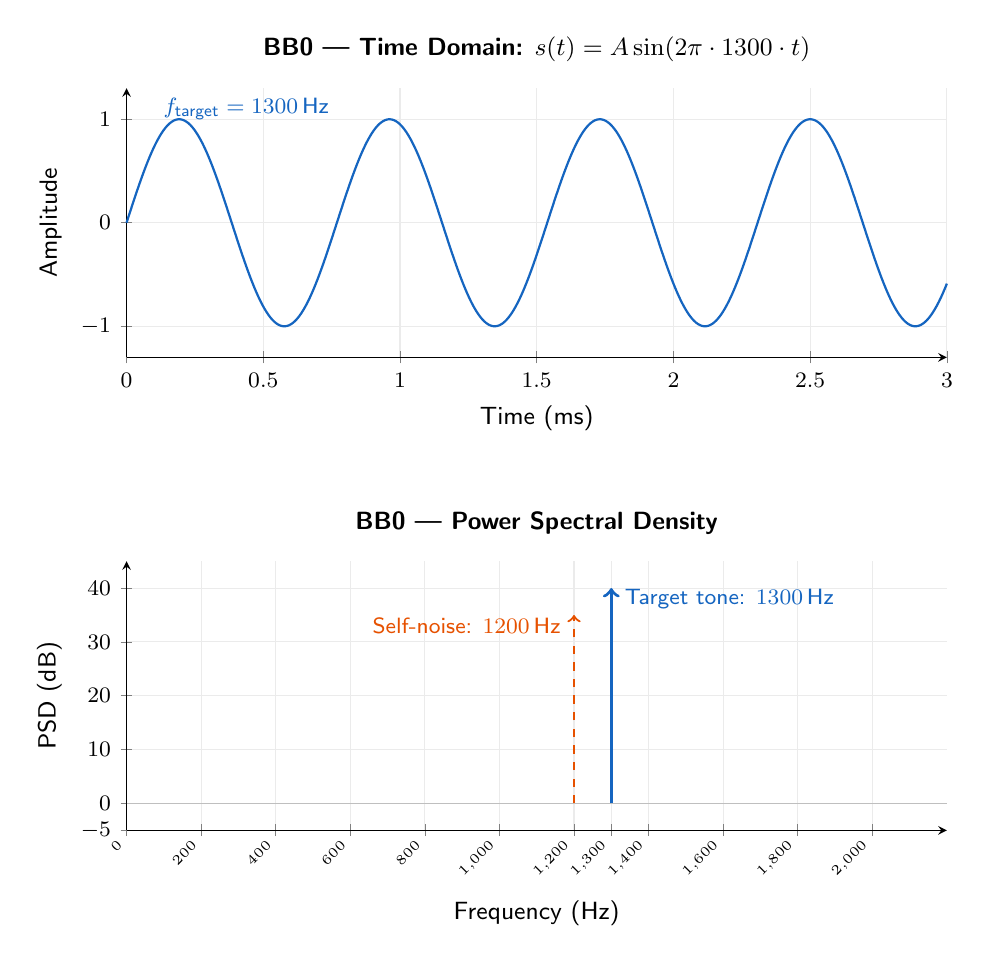
\begin{tikzpicture}
\begin{axis}[
  %% ── layout ────────────────────────────────────────────────────────
  name=timeplot,
  width=12cm, height=5cm,
  xmin=0, xmax=3,
  ymin=-1.3, ymax=1.3,
  xlabel={Time (ms)},
  ylabel={Amplitude},
  title={\textbf{BB0 — Time Domain:}
         $s(t) = A\sin\!\left(2\pi \cdot 1300 \cdot t\right)$},
  xtick={0,0.5,1.0,1.5,2.0,2.5,3.0},
  ytick={-1,0,1},
  grid=both, grid style={black!8},
  axis lines=left,
  tick label style={font=\sffamily\footnotesize},
  label style={font=\sffamily\small},
  title style={font=\sffamily\small},
  clip=false
]
  %% 1300 Hz sine over 3 ms; t in ms → multiply by 1e-3 for seconds
  %% 1300 * 1e-3 = 1.3 cycles per ms
  \addplot[toneBlue, thick, smooth, samples=400, domain=0:3]
      {sin(deg(2*pi*1.3*x))};
  \node[toneBlue, font=\sffamily\footnotesize, anchor=west] at (axis cs:0.1,1.1)
      {$f_{\text{target}} = 1300\,\text{Hz}$};
\end{axis}

\begin{axis}[
  %% ── layout ────────────────────────────────────────────────────────
  name=psdplot,
  at={(timeplot.below south west)}, anchor=above north west,
  yshift=-0.8cm,
  width=12cm, height=5cm,
  xmin=0, xmax=2200,
  ymin=-5, ymax=45,
  xlabel={Frequency (Hz)},
  ylabel={PSD (dB)},
  title={\textbf{BB0 — Power Spectral Density}},
  xtick={0,200,400,600,800,1000,1200,1300,1400,1600,1800,2000},
  xticklabel style={rotate=45, anchor=east, font=\sffamily\tiny},
  ytick={-5,0,10,20,30,40},
  grid=both, grid style={black!8},
  axis lines=left,
  tick label style={font=\sffamily\footnotesize},
  label style={font=\sffamily\small},
  title style={font=\sffamily\small},
  clip=false
]
  %% Flat noise floor at 0 dB
  \addplot[black!25, thin, domain=0:2200] {0};

  %% Target tone spike at 1300 Hz (drawn as a thick vertical line + arrowhead)
  \addplot[toneBlue, very thick, ->]
      coordinates {(1300, 0) (1300, 40)};
  \node[toneBlue, anchor=west, font=\sffamily\footnotesize]
      at (axis cs:1310, 38) {Target tone: $1300\,\text{Hz}$};

  %% Self-noise reference dashed line at 1200 Hz
  \addplot[selfOrange, dashed, thick, ->]
      coordinates {(1200, 0) (1200, 35)};
  \node[selfOrange, anchor=east, font=\sffamily\footnotesize]
      at (axis cs:1190, 33) {Self-noise: $1200\,\text{Hz}$};

\end{axis}
\end{tikzpicture}
\end{document}
